%%%%%%%%%%%%%%%%%%%%%%%%%%%%%%%%%%%%%%%%%%%%%%%%%%%%%%%%%%%%%%%%%%%%%%%%%%%%%%%%
%% MASTER'S THESIS                                                            %%
%%                                                                            %% 
%% Title (en): Multi-Agent Systems and Organizations                          %%
%% Title (cs): Multiagentní systémy a organizace                              %%
%%                                                                            %%
%% Author: Bc. Lukáš Kúdela                                                   %%
%% Supervisor: Prof. RNDr. Petr Štěpánek, DrSc.                               %%
%%                                                                            %%
%% Academic year: 2011/2012                                                   %%
%%%%%%%%%%%%%%%%%%%%%%%%%%%%%%%%%%%%%%%%%%%%%%%%%%%%%%%%%%%%%%%%%%%%%%%%%%%%%%%%

\section{Example 3: Sealed-Bid Auction}

% Section intro - 'Sealed-Bid Auction' organization
This example demonstrates a relatively complex organization---\textit{sealed-bid auction}.
% 'Sealed-Bid Auction' organization - purpose
The purpose of this organization is to facilitate sealed-bid auction by bringing together several agents: one agent \textit{auctions} an item and the other agents \textit{bid} for it.

% Sealed-bid auction
A \textit{sealed-bid auction} is a type of auction in which bidders simultaneously submit bids to the auctioneer without knowledge of the amount bid by other participants.
% First-price (envelope) vs. second-price (Vickrey) auction
Two sub-types of a sealed-bid auction are supported, depending on whether the winner pays the amount bid---a \textit{first-price auction}, also called an \textit{envelope auction}---or an amount equal to the next highest bid---\textit{a second-price auction}, also known as a \textit{Vickrey auction}.

% Open auction
% Ascending price (English) vs. descending price (Dutch) auction

% Assumptions
In this example, agents participate in an envelope auction selling and buying famous paintings, but it should be obvious that any of the two auction types could be used to sell any items.

%%%%%%%%%%%%%%%%%%%%%%%%%%%%%%%%%%%%%%%%%%%%%%%%%%%%%%%%%%%%%%%%%%%%%%%%%%%%%%%%
\subsection*{Specification}

%%%%%%%%%%%%%%%%%%%%%%%%%%%%%%%%%%%%%%%%%%%%%%%%%%%%%%%%%%%%%%%%%%%%%%%%%%%%%%%%
\subsubsection*{Organization Part}

% 'Auction' organizaiton type
The \textit{Auction} organization type (modelled by the \texttt{Auction\_Organization} agent class) contains two roles---\textit{Auctioneer} and \textit{Bider}---and two protocols---\textit{Envelope auction} and  \textit{Vickrey auction}.
% 'auction' organization
\textit{Auction} has one instance in the running MAS: the \textit{auction} organization (modelled by the \texttt{auction\_Organization} agent instance).

% 'Auctioneer' role
The \textit{Auctioneer} role (modelled by the \texttt{Auctioneer\_Role} agent class) can auction an item in an auction.
% 'Auctioneer' role - multiplicity, competences & responsibilities
The \textit{Auctioneer} role is a \textit{single} role.
It has one competence---\textit{Auction}---and no responsibilities.

% 'Auction' competence
The \textit{Auction} competence (modelled by the \texttt{Auction\_Competence} class) is a competence to auction an item.
% 'Auction' competence - argument & result
It has several arguments--mainly the name of the item and the \textit{reserve price}\footnote{The smallest price at which a seller is willing to sell an item.}---and several results---particularly the winner's AID and \textit{hammer price}\footnote{The price at which an item is eventually sold.}.

% 'Bidder' role
The \textit{Bidder} role (modelled by the \texttt{Bidder\_Role} class) can bid for an item in an auction.
% 'Bidder' role - multiplicity, competences & responsibilities
The \textit{Bidder} role is a \textit{multiple} role.
It has no competences and one responsibility---\textit{Bid}.

% 'Bid' responsibility
The \textit{Bid} responsibility (modelled by the \texttt{Bid\_Responsibility} class) is a responsibility to bid for an item.
% 'Bid' responsibility - argument & result
It has several arguments---mainly the name of the item---and several results---the bid amount in particular.

%%%%%%%%%%%%%%%%%%%%%%%%%%%%%%%%%%%%%%%%%%%%%%%%%%%%%%%%%%%%%%%%%%%%%%%%%%%%%%%%
\subsubsection*{Protocol Part}

% 'Envelope acution' protocol
The \textit{Envelope auction} protocol (modelled by the \texttt{EnvelopeAuctionProtocol} class) is a protocol defining an envelope auction by which an \textit{Auctioneer} (the initiator party, modelled by the \texttt{EnvelopeAuction\_InitiatorParty} class) can determine the best buyer from among the \textit{Bidders} (responder party, modelled by the \texttt{EnvelopeAuction\_RespoderParty} class).

% Vickrey auction protocol
The \textit{Vickrey auction} protocol (modelled by the \texttt{VickreyAuctionProtocol} class) is a protocol defining a Vickrey auction by which an \textit{Auctioneer} (the initiator party, modelled by the \texttt{VickreyAuction\_InitiatorParty} class) can choose the best buyer from among the \textit{Bidders} (responder party, modelled by the \texttt{VickreyAuction\_RespoderParty} class).

%% English auction protocol
%The \textit{English auction} protocol (modelled by the \texttt{EnglishAuctionProtocol} class) is a protocol defining an English auction by which an \textit{Auctioneer} (the initiator party, modelled by the \texttt{EnglishAuction\_InitiatorParty} class) can determine the best buyer from among the \textit{Bidders} (responder party, modelled by the \texttt{EnglishAuction\_RespoderParty} class).

%% Dutch auction protocol
%The \textit{Dutch auction} protocol (modelled by the \texttt{DutchAuctionProtocol} class) is a protocol defining a Dutch auction by which an \textit{Auctioneer} (the initiator party, modelled by the \texttt{DutchAuction\_InitiatorParty} class) can determine the best buyer from among the \textit{Bidders} (responder party, modelled by the \texttt{DutchAuction\_RespoderParty} class).

% 'Auction call-for-proposals' message
The \textit{Auction call-for-proposals (CFP)} message (modelled by the \texttt{AuctionCFPMessage} class) is a message sent by an \textit{Auctioneer} to all \textit{Bidders} calling for proposals for the item's price (bids).

% 'Bid propose' message
The \textit{Bid propose} message (modelled by the \texttt{BidProposeMessage} class) is a message sent by a \textit{Bidder} to an \textit{Auctioneer} proposing a price for the item (bid).

%%%%%%%%%%%%%%%%%%%%%%%%%%%%%%%%%%%%%%%%%%%%%%%%%%%%%%%%%%%%%%%%%%%%%%%%%%%%%%%%
\subsubsection*{Player Part}

% 'Participant' player type
The \textit{Participant} player type (modelled by the \texttt{Participant\_Player} agent class) is a player capable of biding for an item.
\textit{Participant} has three instances in the running MAS: \textit{player1}, \textit{player2} and \textit{player3}.
All of them intend to enact both the \textit{Auctioneer} and \textit{Bidder} roles in the \textit{auction} organization and exercise the \textit{Auctioneer} role's \textit{Auction} competence---to auction an item to the players of the \textbf{Bidder} role.
They also intend to fulfil the \textit{Bidder} role's \textit{Bid} responsibility---to bid for an item auctioned by the player of the \textit{Auctioneer} role.
% 'player1' player
\textit{player1} (modelled by the \texttt{player1} agent instance) intends to play the role of \textbf{Auctioneer} in the \textit{first} round and be a \textbf{Bidder} in the second and third rounds.
% 'player2' player
\textit{player2} (modelled by the \texttt{player2} agent instance) intends to act as \textit{Auctioneer} in the \textit{second} round and be a \textit{Bidder} in the first and third rounds.
% 'player3' player
\textit{player3} (modelled by the \texttt{player3} agent instance) intends to play the role of \textit{Auctioneer} in the \textit{third} round and be the \textit{Bidder} in the first and second rounds.

%%%%%%%%%%%%%%%%%%%%%%%%%%%%%%%%%%%%%%%%%%%%%%%%%%%%%%%%%%%%%%%%%%%%%%%%%%%%%%%%
\subsection*{Manifestation} 

%%%%%%%%%%%%%%%%%%%%%%%%%%%%%%%%%%%%%%%%%%%%%%%%%%%%%%%%%%%%%%%%%%%%%%%%%%%%%%%%
\subsubsection*{Stage 3: Competence and Responsibility Invocation}

% Figure: Stage 3: Competence and responsibility invocation
\begin{figure}[H]
	\centering
	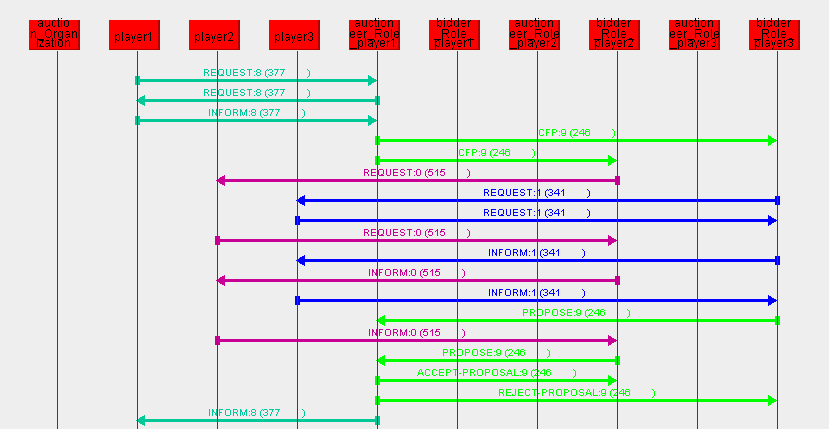
\includegraphics[width=\textwidth]{images/examples/example3-stageA3.png}
	\caption{Stage 3: Competence and responsibility invocation}
	\label{figure:example3-stageA3}
\end{figure}

% Teal
First, \textit{player1} invokes the \textit{Auction} competence for Jason Pollock's \textit{No. 5, 1948} for the reservation price of \$140M\footnote{The actual original price at the private sale of this painting via Sotheby's in 2006.} on its \textit{auctioneer-player1} position (the {\color{teal}{\textbf{teal}}} interaction scenario).

% Green
Next, \textit{auctioneer-player1} calls for proposals for the painting's price from all \textit{Bidder} positions (the {\color{green}{\textbf{green}}} interaction scenario).

% Purple & blue
To obtain their proposals, the \textit{bidder-player2} and \textit{bidder-player3} positions invoke the \textit{Bid} responsibility on their \textit{player2} and \textit{player3} respectively (the {\color{purple}{\textbf{purple}}} and {\color{blue}{\textbf{blue}}} interaction scenarios respectively).
\textit{player2} bids \$156.8M\footnote{The actual adjusted price at the private sale of this painting.} and \textit{player3} makes a bid of \$155.8M.

% Green (again)
\textit{bidder-player2} and \textit{bidder-player3} propose their bids to \textit{auctioneer-player1} (the {\color{green}{\textbf{green}}} interaction scenario again), who determines the auction winner and the hammer price and also determines whether the auction is ultimately successful, i.e. whether the hammer price is at least the reservation price.
The winner is the highest-bidding bidder---\textit{bidder-player2}.
Because this is an envelope auction, the hammer price is the highest amount bid--- \$156.8M.
Since the hammer price is way above the reservation price, the auction is successful.

% Green (still)
Next, \textit{auctioneer-player1} informs the winner---\textit{bidder-player2}---that his proposal has been accepted and all other bidders---\textit{bidder-player3}---that their proposal has been rejected (still the {\color{green}{\textbf{green}}} interaction scenario).

% Teal (again)
Finally, \textit{auctioneer-player1} informs \textit{player1} about the outcome of the auction---whether it was successful or not and in case it was, who is the winner and what is the hammer price (the {\color{teal}{\textbf{teal}}} interaction scenario again).